% Slide 1: Title
{
\setbeamertemplate{headline}{}
\setbeamertemplate{footline}{}
\begin{frame}[plain]
  \vspace{0.4cm}
  \begin{center}
    {\fontsize{8.5}{11}\selectfont\color{subgray}دانشگاه مانهایم \ | \ \lr{IE500} داده‌کاوی \ | \ مقدمه و ساختار درس \ | \ نسخه \lr{01.09.2024}}\\[0.2cm]
    {\fontsize{10}{12}\selectfont\color{mannheimgold}\textbf{گروه علوم داده و وب}}\\[0.3cm]
    {\fontsize{20}{24}\selectfont\color{mannheimblue}\textbf{داده‌کاوی (\lr{IE500})}}\\[0.2cm]
    {\fontsize{13}{16}\selectfont\color{mannheimteal}\textbf{فصل ۱: مقدمه و ساختار درس}}\\[0.3cm]
    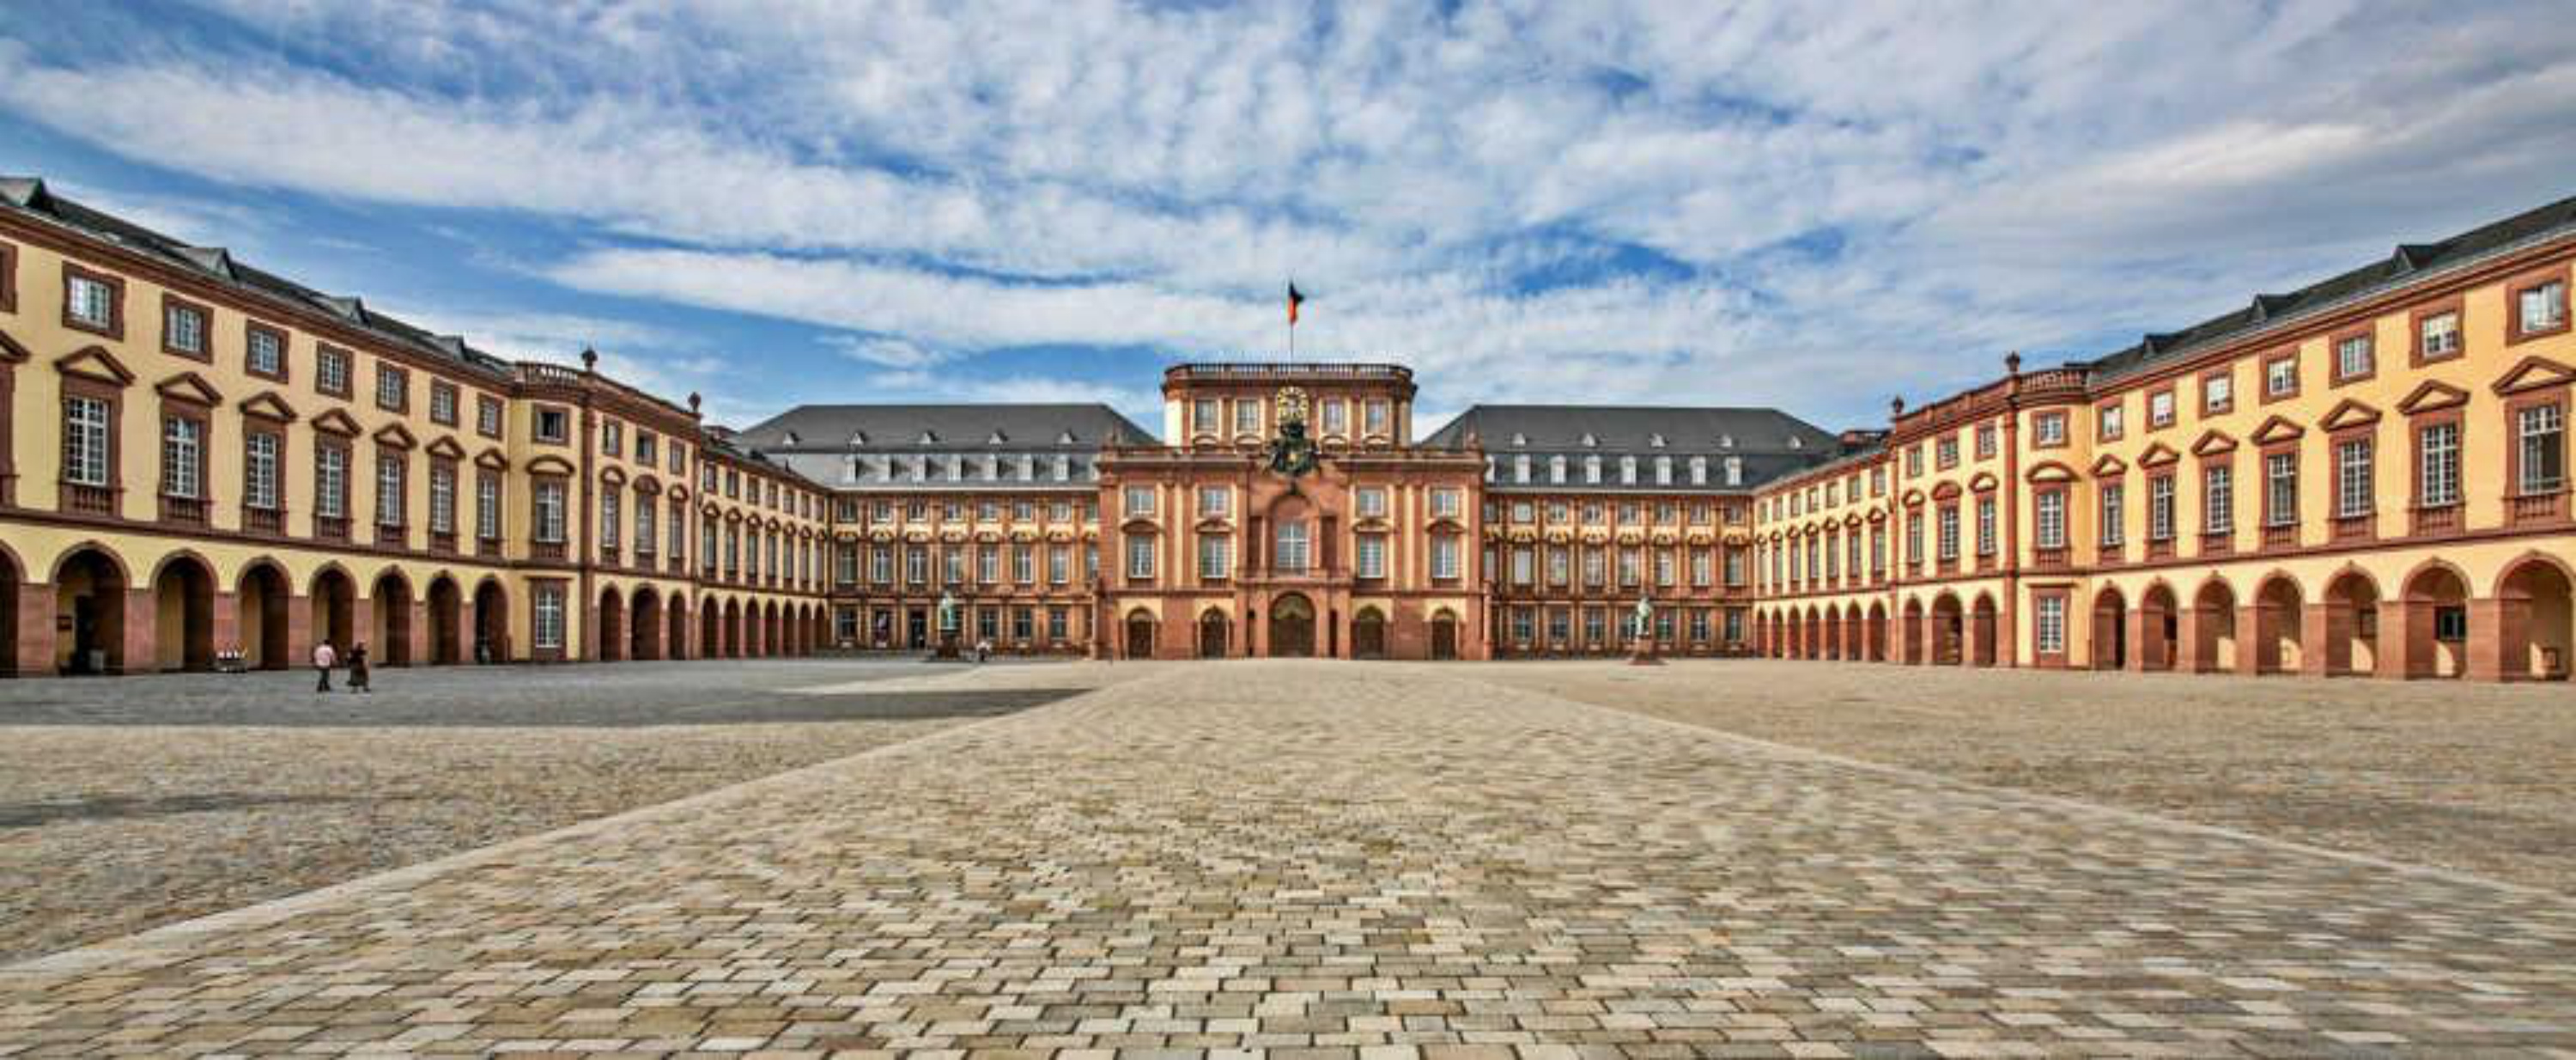
\includegraphics[width=\textwidth,height=2.8cm,keepaspectratio]{images/img_p01_1_20.jpeg}\\[0.3cm]
    
\includegraphics[height=0.8cm]{images/mannheim_logo.png}
  \end{center}
\end{frame}
}

% Slide 2: Hello - Dr. Sven Hertling
\begin{frame}{معرفی مدرس درس}
\framesubtitle{\lr{Dr. Sven Hertling}}
\begin{columns}[T,onlytextwidth]
\begin{column}{0.68\textwidth}
\begin{itemize}
  \item \textbf{دکتر اسون هرتلینگ} (\lr{Dr. Sven Hertling})
  \begin{itemize}
    \item استاد مدعو و جانشین کرسی علوم داده (\lr{Substitute Professor for Data Science})
  \end{itemize}
  \vspace{0.2cm}
  \item \textbf{حوزه‌های پژوهشی:}
  \begin{itemize}
    \item ادغام گراف‌های دانش (\lr{Knowledge Graph Integration})
    \item ترکیب گراف‌های دانش با مدل‌های زبانی بزرگ (\lr{KGs with LLMs})
    \item استخراج اطلاعات (\lr{Information Extraction})
  \end{itemize}
  \vspace{0.2cm}
  \item \textbf{اتاق:} \lr{B6 26, B0.21}
  \item \textbf{ایمیل:} \lr{sven.hertling@uni-mannheim.de}
  \item \textbf{مسئولیت:} ارائه جلسات تئوری و اصلی درس (\lr{Lectures})
\end{itemize}
\end{column}
\begin{column}{0.28\textwidth}
\begin{center}
  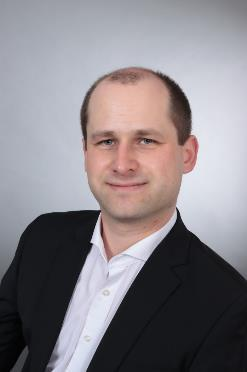
\includegraphics[width=\textwidth,height=4.8cm,keepaspectratio]{images/img_p02_1_34.jpeg}
\end{center}
\end{column}
\end{columns}
\end{frame}

% Slide 3: Hello - Andreea Iana
\begin{frame}{معرفی دستیاران آموزشی}
\framesubtitle{\lr{M.Sc. Andreea Iana}}
\begin{columns}[T,onlytextwidth]
\begin{column}{0.68\textwidth}
\begin{itemize}
  \item \textbf{آندریا یانا} (\lr{M.Sc. Andreea Iana})
  \begin{itemize}
    \item پژوهشگر و دستیار تحقیق (\lr{Graduate Research Associate})
  \end{itemize}
  \vspace{0.2cm}
  \item \textbf{حوزه‌های پژوهشی:}
  \begin{itemize}
    \item سامانه‌های توصیه‌گر (\lr{Recommender Systems})
    \item بازیابی اطلاعات (\lr{Information Retrieval})
    \item پردازش زبان طبیعی (\lr{Natural Language Processing})
  \end{itemize}
  \vspace{0.2cm}
  \item \textbf{اتاق:} \lr{B6 26, B 0.18}
  \item \textbf{ایمیل:} \lr{andreea.iana@uni-mannheim.de}
  \item \textbf{مسئولیت:} تدریس یکی از گروه‌های تمرین و هدایت پروژه‌های دانشجویی
\end{itemize}
\end{column}
\begin{column}{0.28\textwidth}
\begin{center}
  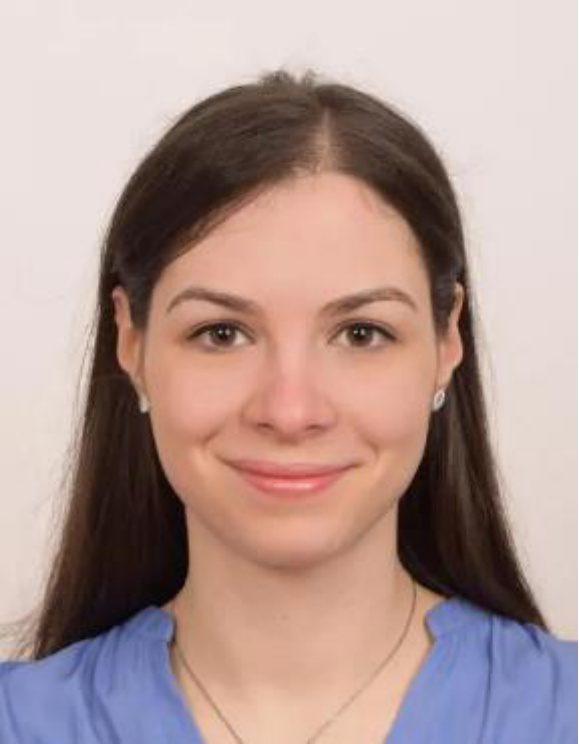
\includegraphics[width=\textwidth,height=4.8cm,keepaspectratio]{images/img_p03_1_38.jpeg}
\end{center}
\end{column}
\end{columns}
\end{frame}

% Slide 4: Hello - Franz Krause
\begin{frame}{معرفی دستیاران آموزشی}
\framesubtitle{\lr{M.Sc. Franz Krause}}
\begin{columns}[T,onlytextwidth]
\begin{column}{0.68\textwidth}
\begin{itemize}
  \item \textbf{فرانتس کراوزه} (\lr{M.Sc. Franz Krause})
  \begin{itemize}
    \item پژوهشگر و دستیار تحقیق (\lr{Graduate Research Associate})
  \end{itemize}
  \vspace{0.15cm}
  \item \textbf{حوزه‌های پژوهشی:}
  \begin{itemize}
    \item کاربردهای یادگیری ماشین روی داده‌های پیوندی (\lr{ML on Linked Data})
    \item پویایی بازنمایی‌های تعبیه گراف دانش (\lr{KG Embeddings})
    \item کاربرد و استقرار گراف دانش در محیط‌های صنعتی
    \item نظریه گراف کاربردی (\lr{Applied Graph Theory})
  \end{itemize}
  \vspace{0.15cm}
  \item \textbf{اتاق:} \lr{B6 26, B 0.02}
  \item \textbf{ایمیل:} \lr{franz.krause@uni-mannheim.de}
  \item \textbf{مسئولیت:} تدریس یکی از گروه‌های تمرین و هدایت پروژه‌های دانشجویی
\end{itemize}
\end{column}
\begin{column}{0.28\textwidth}
\begin{center}
  
\includegraphics[width=\textwidth,height=4.8cm,keepaspectratio]{images/img_p04_1_42.jpeg}
\end{center}
\end{column}
\end{columns}
\end{frame}

% Slide 5: Hello - Aaron Steiner
\begin{frame}{معرفی دستیاران آموزشی}
\framesubtitle{\lr{M.Sc. Aaron Steiner}}
\begin{columns}[T,onlytextwidth]
\begin{column}{0.68\textwidth}
\begin{itemize}
  \item \textbf{آرون اشتاینر} (\lr{M.Sc. Aaron Steiner})
  \begin{itemize}
    \item پژوهشگر و دستیار تحقیق (\lr{Graduate Research Associate})
  \end{itemize}
  \vspace{0.2cm}
  \item \textbf{حوزه‌های پژوهشی:}
  \begin{itemize}
    \item تطبیق موجودیت‌ها با مدل‌های زبانی (\lr{Entity Matching using LLMs})
    \item تنظیم دقیق مدل‌های زبانی بزرگ (\lr{Fine-tuning LLMs})
    \item ادغام داده‌ها (\lr{Data Integration})
  \end{itemize}
  \vspace{0.2cm}
  \item \textbf{اتاق:} \lr{B6 26, C 1.04}
  \item \textbf{ایمیل:} \lr{aaron.steiner@uni-mannheim.de}
  \item \textbf{مسئولیت:} تدریس یکی از گروه‌های تمرین و هدایت پروژه‌های دانشجویی
\end{itemize}
\end{column}
\begin{column}{0.28\textwidth}
\begin{center}
  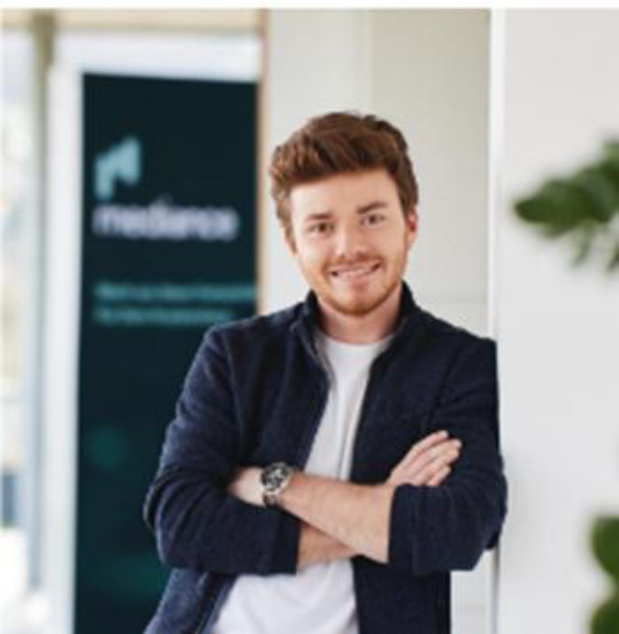
\includegraphics[width=\textwidth,height=4.8cm,keepaspectratio]{images/img_p05_1_46.jpeg}
\end{center}
\end{column}
\end{columns}
\end{frame}

% Slide 6: Course Organization
\begin{frame}{سازماندهی درس -- جلسات کلاس تئوری}
\begin{columns}[T,onlytextwidth]
\begin{column}{0.62\textwidth}
\begin{itemize}
  \item \textbf{ثبت‌نام} (\lr{Registration})
  \begin{itemize}
    \item ثبت‌نام رسمی از طریق پورتال \lr{Portal2}
    \item عضویت خودکار در سامانه آموزشی \lr{ILIAS}
  \end{itemize}
  \vspace{0.25cm}
  \item \textbf{کلاس درس تئوری} (\lr{Lecture})
  \begin{itemize}
    \item \textbf{زمان:} چهارشنبه‌ها، ساعت \lr{10:15 -- 11:45}
    \item \textbf{مکان:} اتاق \lr{B144}، ساختمان \lr{A 5,6} بخش \lr{B}
    \item معرفی اصول و روش‌های بنیادین داده‌کاوی
    \item نحوه ارزیابی و اعتبارسنجی مدل‌های آموخته‌شده
    \item ارائه مثال‌های کاربردی و سناریوهای واقعی در صنعت
  \end{itemize}
\end{itemize}
\end{column}
\begin{column}{0.35\textwidth}
\begin{center}
  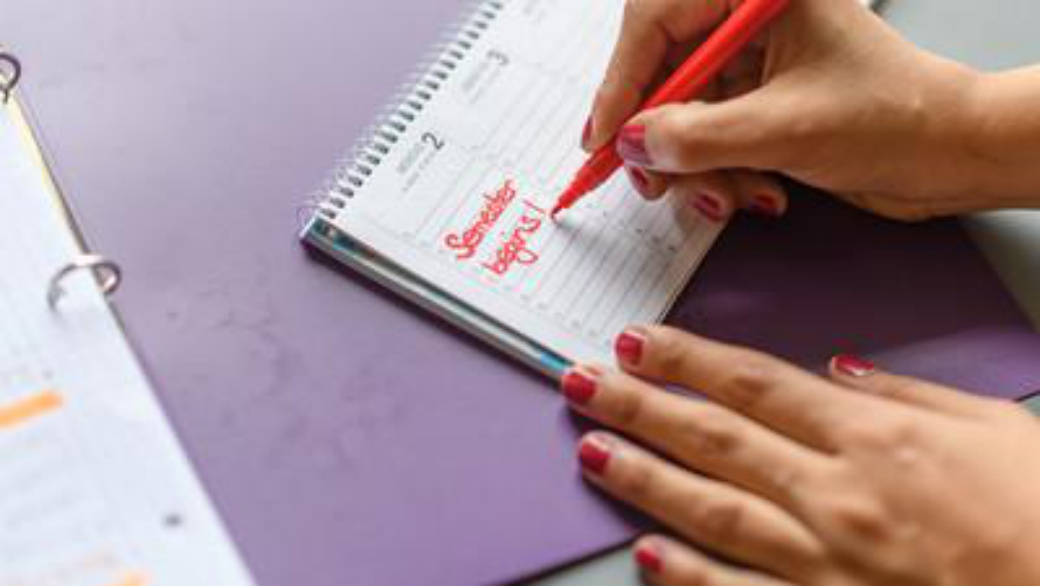
\includegraphics[width=\textwidth,height=3.8cm,keepaspectratio]{images/img_p06_1_56.jpeg}
\end{center}
\end{column}
\end{columns}
\end{frame}

% Slide 7: Course Organization - Material
\begin{frame}{سازماندهی درس -- منابع و سامانه‌های آموزشی}
\begin{columns}[T,onlytextwidth]
\begin{column}{0.62\textwidth}
\begin{itemize}
  \item \textbf{وب‌سایت رسمی درس} (\lr{Course Webpage})
  \begin{itemize}
    \item ارائه اطلاعات به‌روز، اسلایدهای آموزشی و ویدیوهای درس
    \item \lr{\footnotesize https://www.uni-mannheim.de/dws/teaching/}
  \end{itemize}
  \vspace{0.25cm}
  \item \textbf{سامانه آموزش الکترونیکی \lr{ILIAS}}
  \begin{itemize}
    \item پیوند: \lr{https://ilias.uni-mannheim.de/}
    \item دریافت تمرین‌ها و مجموعه‌داده‌ها
    \item تالارهای گفتگو و پرسش‌وپاسخ (\lr{Discussion Forum})
    \item تحویل پروژه‌های تیمی و جلسات راهنمایی مربیان
  \end{itemize}
\end{itemize}
\end{column}
\begin{column}{0.35\textwidth}
\begin{center}
  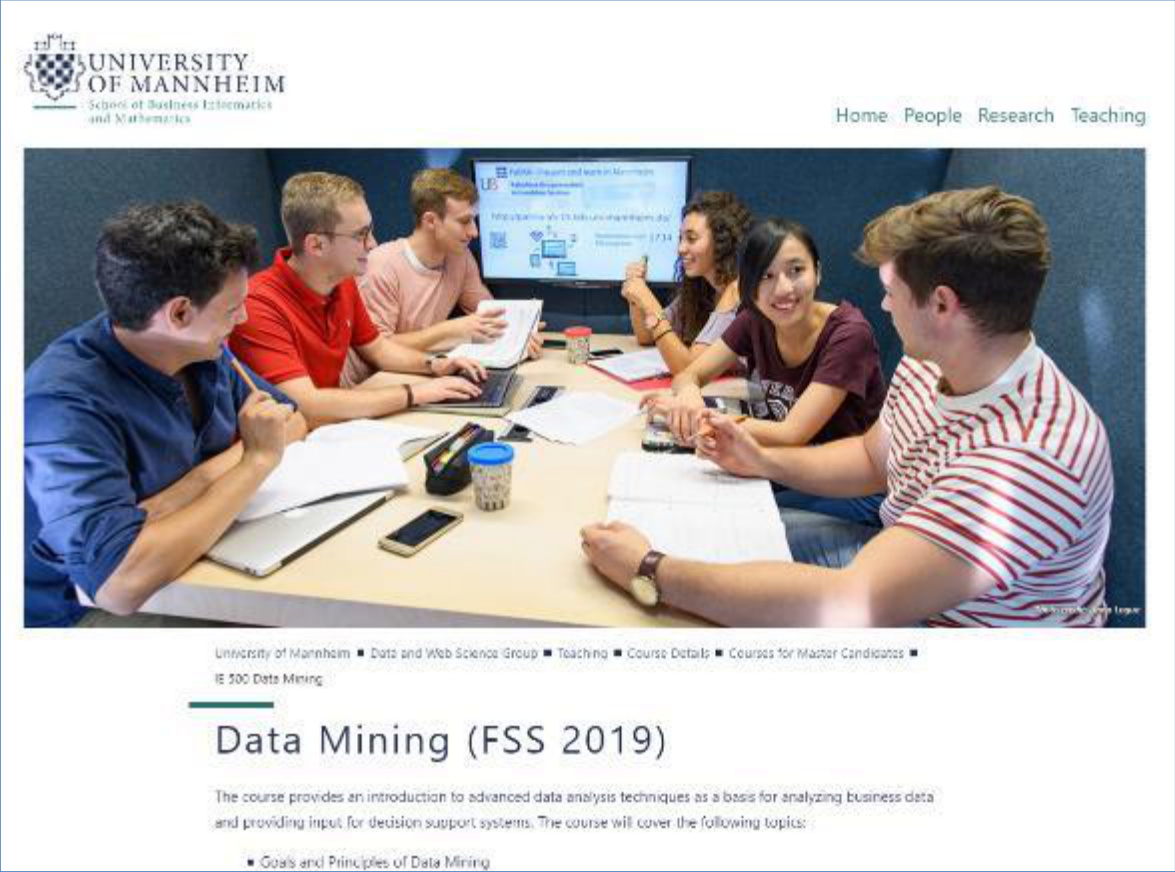
\includegraphics[width=0.85\textwidth]{images/img_p07_2_64.jpeg}\\[0.15cm]
  
\includegraphics[width=0.35\textwidth]{images/img_p07_3_65.png}\\[0.15cm]
  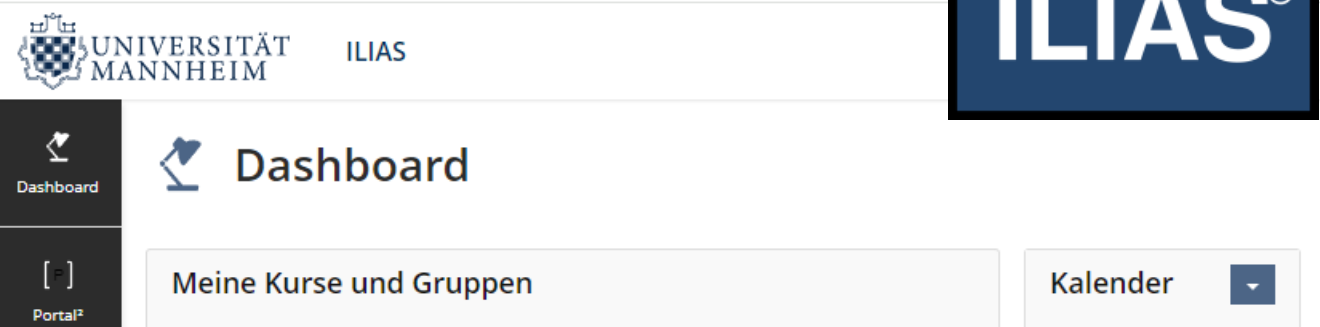
\includegraphics[width=0.85\textwidth]{images/img_p07_1_63.png}
\end{center}
\end{column}
\end{columns}
\end{frame}

% Slide 8: Course Organization - Material (Online Lecture)
\begin{frame}{سازماندهی درس -- جلسات آموزش برخط}
\begin{columns}[T,onlytextwidth]
\begin{column}{0.5\textwidth}
\begin{itemize}
  \item \textbf{کلاس‌های مجازی} (\lr{Online Lecture})
  \begin{itemize}
    \item بخش رسمی و الزامی از برنامه آموزشی درس
    \item پوشش سرفصل‌های مکمل داده‌کاوی
    \item کاملاً مرتبط با مباحث تمرین‌ها و سؤالات آزمون نهایی
    \item امکان مرور چندباره و یادگیری با سرعت شخصی
  \end{itemize}
\end{itemize}
\end{column}
\begin{column}{0.48\textwidth}
\begin{center}
  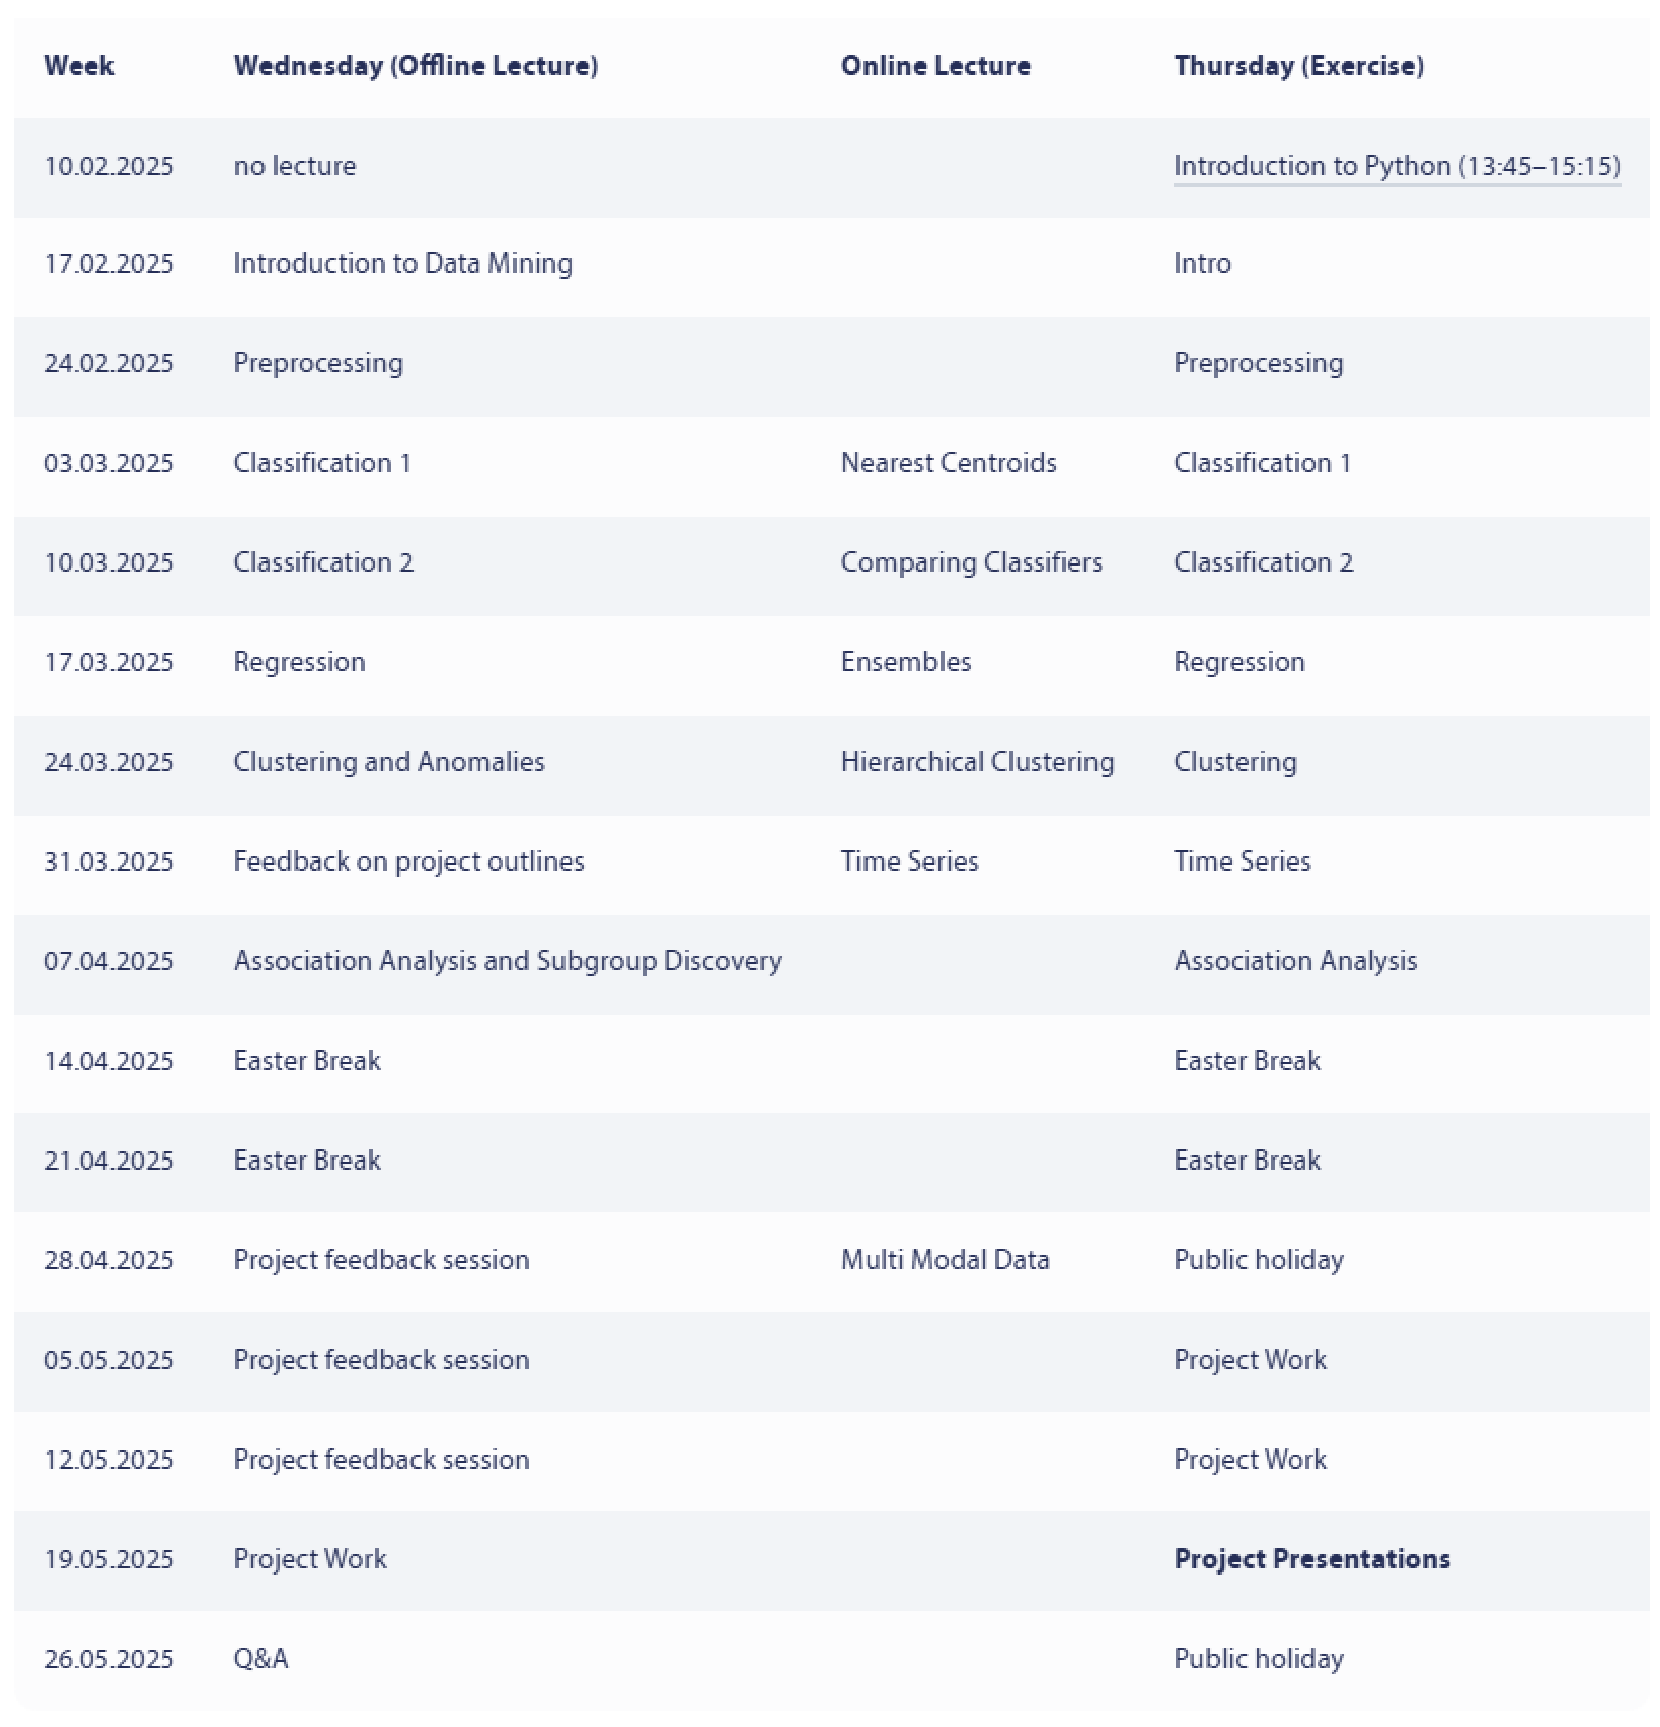
\includegraphics[width=0.75\textwidth,height=2cm,keepaspectratio]{images/img_p08_2_70.png}\\[0.15cm]
  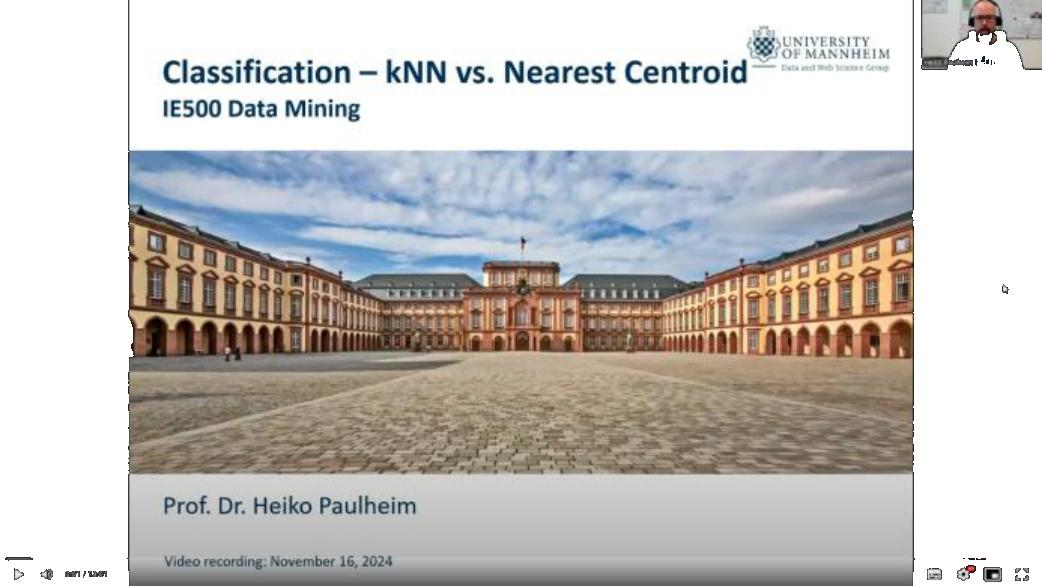
\includegraphics[width=0.65\textwidth,height=1.6cm,keepaspectratio]{images/img_p08_1_69.jpeg}
\end{center}
\end{column}
\end{columns}
\end{frame}

% Slide 9: Course Organization - Exercise
\begin{frame}{سازماندهی درس -- گروه‌های حل تمرین}
\begin{columns}[T,onlytextwidth]
\begin{column}{0.62\textwidth}
\begin{itemize}
  \item \textbf{جلسات تمرین عملی} (\lr{Exercise Groups})
  \begin{itemize}
    \item آزمایش و کار با داده‌های واقعی در زبان پایتون (\lr{Python})
  \end{itemize}
  \vspace{0.2cm}
  \item \textbf{زمان و مکان جلسات (محتوا یکسان است -- فقط در یک گروه شرکت کنید)}
  \begin{itemize}
    \item پنج‌شنبه، ساعت \lr{10:15 -- 11:45}، اتاق \lr{A104}، ساختمان \lr{B6, 26} بخش \lr{A} (\lr{Aaron})
    \item پنج‌شنبه، ساعت \lr{12:00 -- 13:30}، اتاق \lr{A104}، ساختمان \lr{B6, 26} بخش \lr{A} (\lr{Andreea/Franz})
    \item پنج‌شنبه، ساعت \lr{13:45 -- 15:15}، اتاق \lr{A104}، ساختمان \lr{B6, 26} بخش \lr{A} (\lr{Andreea/Franz})
  \end{itemize}
\end{itemize}
\end{column}
\begin{column}{0.35\textwidth}
\begin{center}
  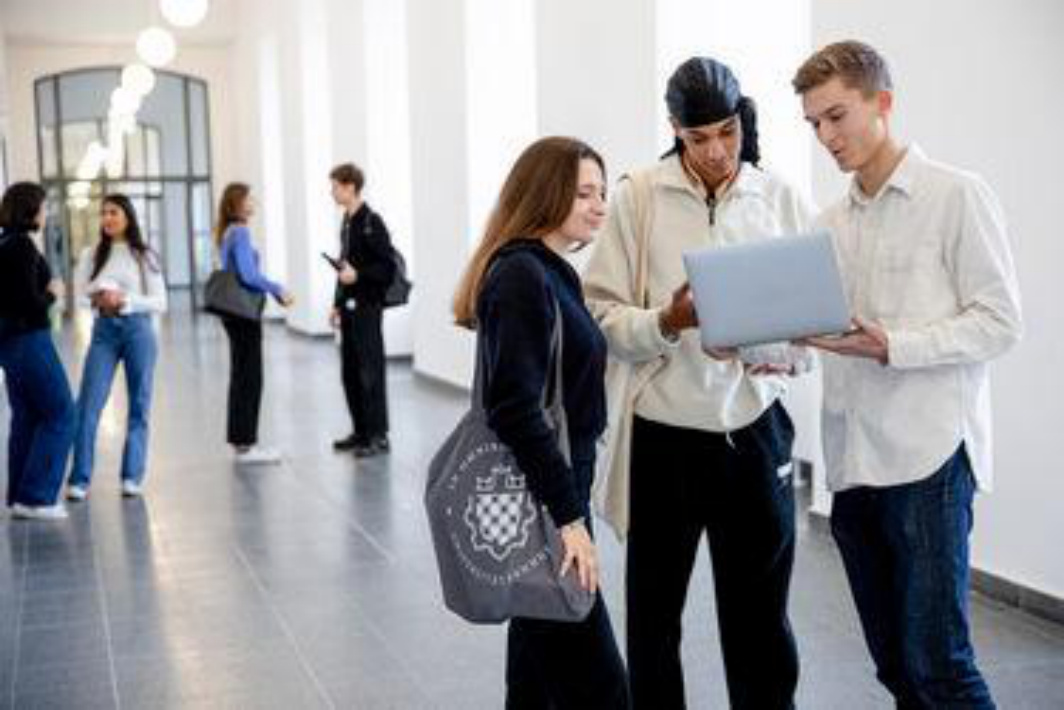
\includegraphics[width=\textwidth,height=4cm,keepaspectratio]{images/img_p09_1_73.jpeg}
\end{center}
\end{column}
\end{columns}
\end{frame}

% Slide 10: Introduction to Python
\begin{frame}{کارگاه مقدماتی برنامه‌نویسی پایتون}
\begin{columns}[T,onlytextwidth]
\begin{column}{0.65\textwidth}
\begin{itemize}
  \item \textbf{جلسه توجیهی پایتون:}
  \begin{itemize}
    \item پنج‌شنبه هفته گذشته، ساعت \lr{13:45 -- 15:15} برگزار گردید
  \end{itemize}
  \vspace{0.2cm}
  \item \textbf{سرفصل‌های ارائه‌شده:}
  \begin{itemize}
    \item نصب و راه‌اندازی محیط (\lr{Anaconda, Jupyter Notebooks})
    \item معرفی فلسفه طراحی زبان پایتون
    \item ساختارهای پایه‌ای برنامه‌نویسی و پردازش داده در پایتون
  \end{itemize}
  \vspace{0.2cm}
  \item \textbf{پشتیبانی و رفع اشکال:}
  \begin{itemize}
    \item راهنمایی در پیکربندی و پاسخ به پرسش‌های دانشجویان
    \item اسلایدهای آموزشی خودآموز در وب‌سایت درس در دسترس است
  \end{itemize}
\end{itemize}
\end{column}
\begin{column}{0.32\textwidth}
\begin{center}
  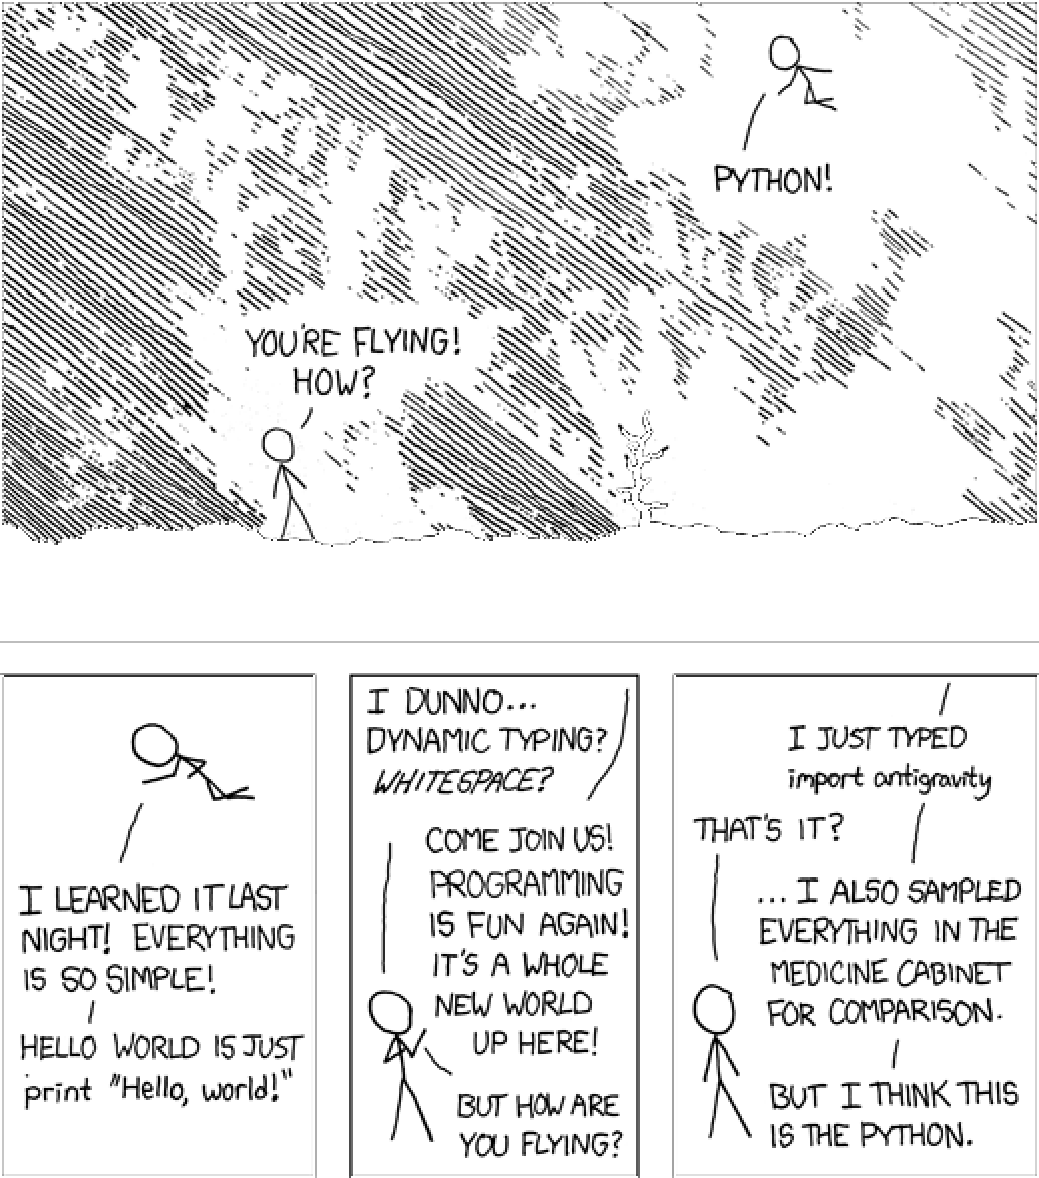
\includegraphics[width=\textwidth,height=3.8cm,keepaspectratio]{images/img_p10_1_76.png}
\end{center}
\end{column}
\end{columns}
\end{frame}

% Slide 11: Usage of ChatGPT
\begin{frame}{استفاده از \lr{ChatGPT} در جلسات تمرین}
\begin{itemize}
  \item \textbf{در جلسات تمرین از \lr{ChatGPT} به صورت هدفمند بهره خواهیم برد برای:}
  \begin{itemize}
    \item \textbf{تحلیل روش‌ها و پارامترها:} هم‌اندیشی درباره انتخاب الگوریتم مناسب و تنظیم هایپرپارامترها در سناریوهای مختلف
    \item \textbf{تولید و خطایابی کد:} نوشتن اسکریپت‌های پایتون و رفع اشکال سریع‌تر در آزمایش‌ها
  \end{itemize}
\end{itemize}
\begin{center}
  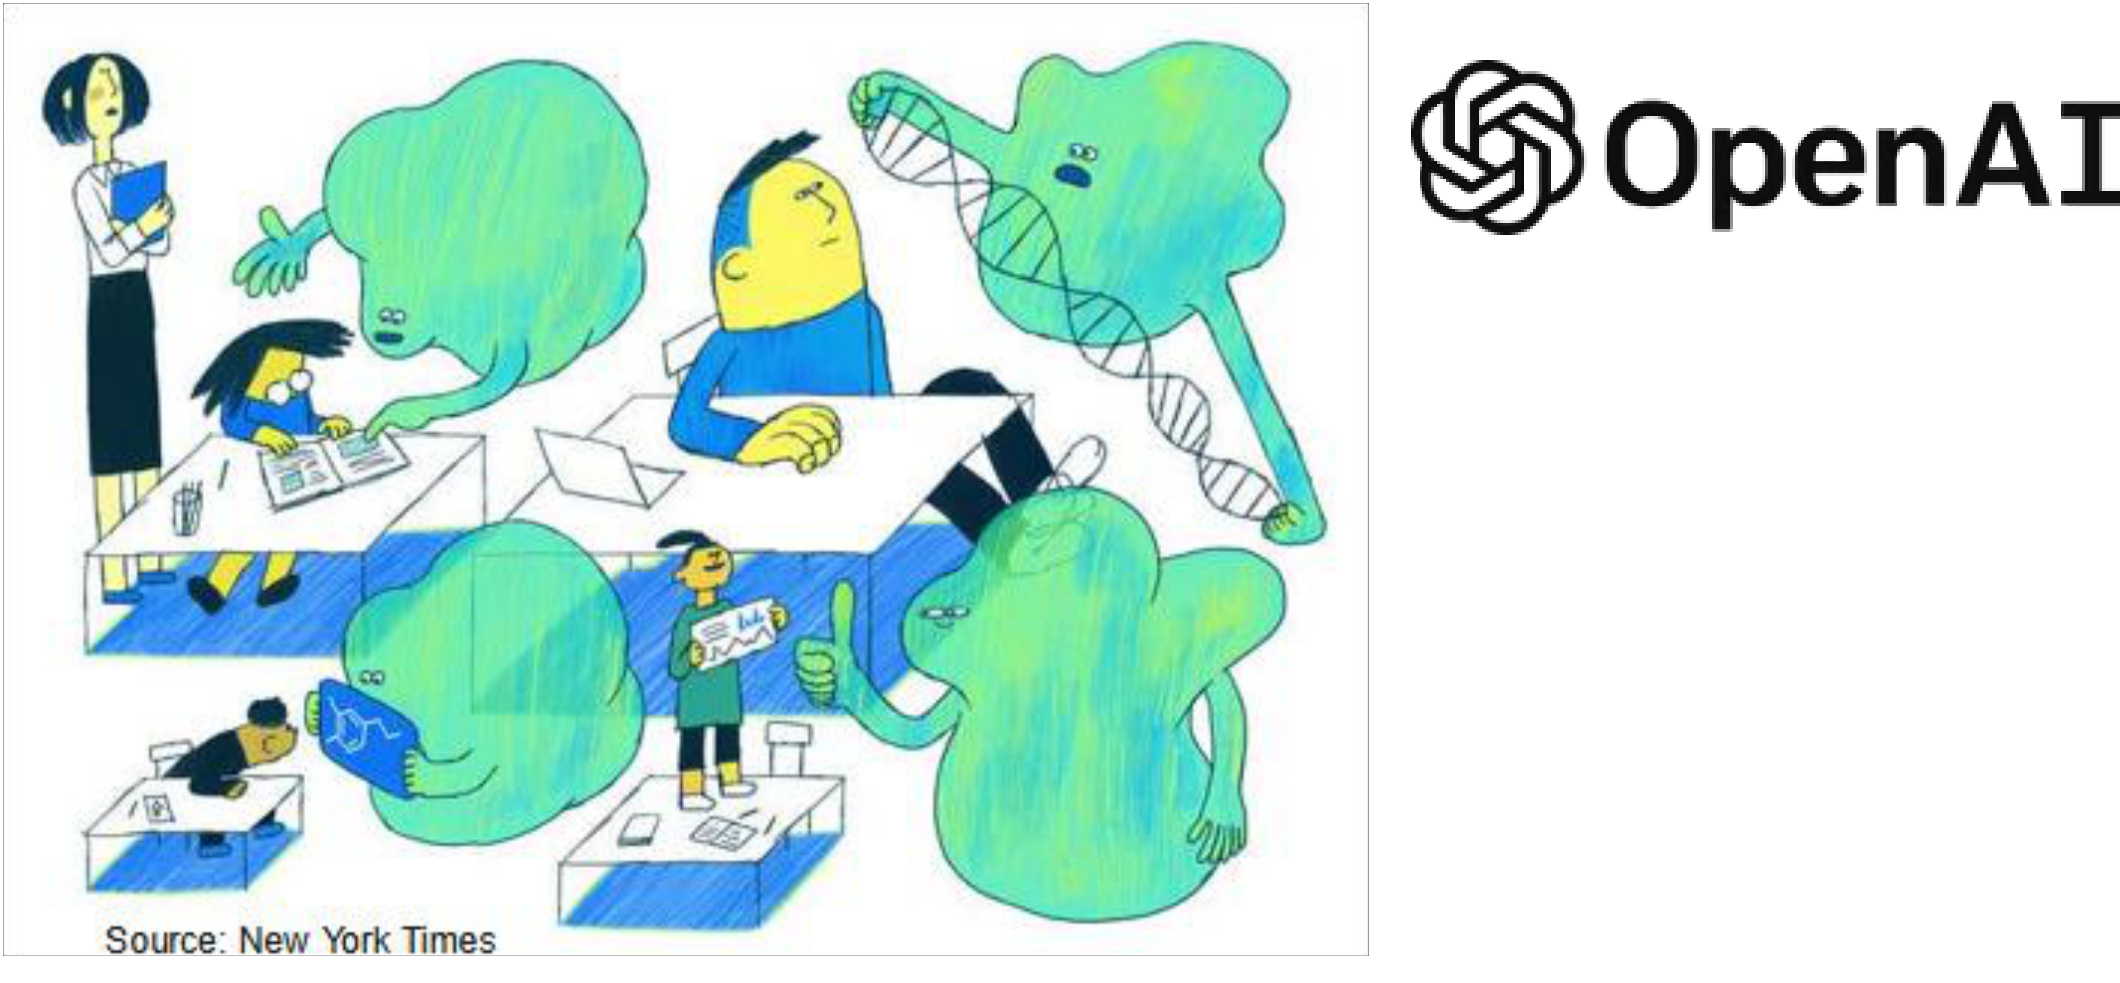
\includegraphics[width=0.72\textwidth,height=3.5cm,keepaspectratio]{images/img_p11_1_79.jpeg}
\end{center}
\end{frame}

% Slide 12: Course Organization - Project
\begin{frame}{سازماندهی درس -- پروژه عملی دانشجویی}
\begin{columns}[T,onlytextwidth]
\begin{column}{0.65\textwidth}
\begin{itemize}
  \item \textbf{اجرای پروژه گروهی} (\lr{Project Work})
  \begin{itemize}
    \item تیم‌های \lr{6} نفره برای اجرای جامع یک پروژه داده‌کاوی واقعی
    \item انتخاب آزاد مجموعه‌داده و مسئله (تعدادی داده نیز پیشنهاد می‌شود)
    \item نگارش گزارش علمی فشرده و ارائه نتایج
  \end{itemize}
  \vspace{0.2cm}
  \item \textbf{مهلت‌های قطعی تحویل} (\lr{Deadlines})
  \begin{itemize}
    \item \textbf{تشکیل و ثبت تیم‌ها:} یکشنبه، \lr{16} مارس، ساعت \lr{23:59}
    \item \textbf{ارسال پروپوزال پروژه} (\lr{Proposal}) -- یکشنبه، \lr{23} مارس، ساعت \lr{23:59}
    \item \textbf{ارسال گزارش نهایی پروژه} -- یکشنبه، \lr{18} مه، ساعت \lr{23:59}
    \item \textbf{ارسال فایل ارائه} (\lr{PDF}) -- چهارشنبه، \lr{21} مه، ساعت \lr{23:59}
  \end{itemize}
\end{itemize}
\end{column}
\begin{column}{0.32\textwidth}
\begin{center}
  
\includegraphics[width=\textwidth,height=3.8cm,keepaspectratio]{images/img_p12_1_83.jpeg}
\end{center}
\end{column}
\end{columns}
\end{frame}

% Slide 13: Course Organization - Exam
\begin{frame}{سازماندهی درس -- مشخصات آزمون کتبی}
\begin{itemize}
  \item \textbf{تاریخ و زمان برگزاری:} پنج‌شنبه، \lr{12} ژوئن \lr{2025} (\lr{Thursday, 12th June 2025})
  \item \textbf{مدت زمان آزمون:} \lr{60} دقیقه
  \item \textbf{ساختار آزمون:} \lr{6} سؤال تشریحی (\lr{6 Open Questions})
  \begin{itemize}
    \item \textbf{سنجش درک مفهومی:} بررسی تسلط عمیق دانشجو بر مباحث تمام فصول اصلی درس
    \item \textbf{تشریح منطق الگوریتم‌ها:} نیازمند توضیح چرایی و چگونگی کارکرد متدها
    \item \textbf{رفتار متدها در شرایط خاص:} بررسی چگونگی واکنش الگوریتم‌ها به الگوها و نویز داده‌ها
    \item \textbf{محاسبات ساده عددی:}
    \begin{itemize}
      \item دانستن فرمول‌های اصلی الزامی است
      \item نیازی به ماشین‌حساب نیست (محاسبات ساده و ذهنی است)
    \end{itemize}
  \end{itemize}
\end{itemize}
\end{frame}

% Slide 14: Course Organization - Exam Rules & Grading
\begin{frame}{سازماندهی درس -- ضوابط آزمون و نمره‌دهی}
\begin{itemize}
  \item \textbf{تنها یک نوبت آزمون در هر نیم‌سال:}
  \begin{itemize}
    \item چون این درس در هر دو ترم (پاییز و بهار) ارائه می‌گردد
    \item نوبت بعدی امتحان در پایان نیم‌سال آینده خواهد بود (بدون آزمون جبرانی یا \lr{Retake} در این ترم!)
  \end{itemize}
  \vspace{0.2cm}
  \item \textbf{شرایط عدم قبولی:}
  \begin{itemize}
    \item در صورت مردودی، باید هم پروژه و هم آزمون را در ترم آینده مجدداً از نو بگذرانید
    \item متأسفانه امکان انتقال نمره پروژه به ترم بعد وجود ندارد
  \end{itemize}
  \vspace{0.2cm}
  \item \textbf{ترکیب نمره نهایی} (\lr{Final Grade})
  \begin{itemize}
    \item \textbf{آزمون کتبی} (\lr{Written Exam}) -- \lr{75\%}
    \item \textbf{گزارش پروژه} (\lr{Project Report}) -- \lr{20\%}
    \item \textbf{ارائه شفاهی پروژه} (\lr{Presentation}) -- \lr{5\%}
  \end{itemize}
\end{itemize}
\end{frame}

% Slide 15: Schedule
\begin{frame}{برنامه زمان‌بندی جلسات درس}
\begin{columns}[T,onlytextwidth]
\begin{column}{0.48\textwidth}
\begin{itemize}
  \item \textbf{تقویم آموزشی ترم:}
  \begin{itemize}
    \item کلیه تاریخ‌ها، مباحث هفتگی و زمان تحویل فازهای پروژه
    \item تمام به‌روزرسانی‌ها به صورت برخط در صفحه خانگی درس قرار می‌گیرد
    \item لطفاً به طور منظم وب‌سایت درس را بررسی فرمایید
  \end{itemize}
\end{itemize}
\end{column}
\begin{column}{0.5\textwidth}
\begin{center}
  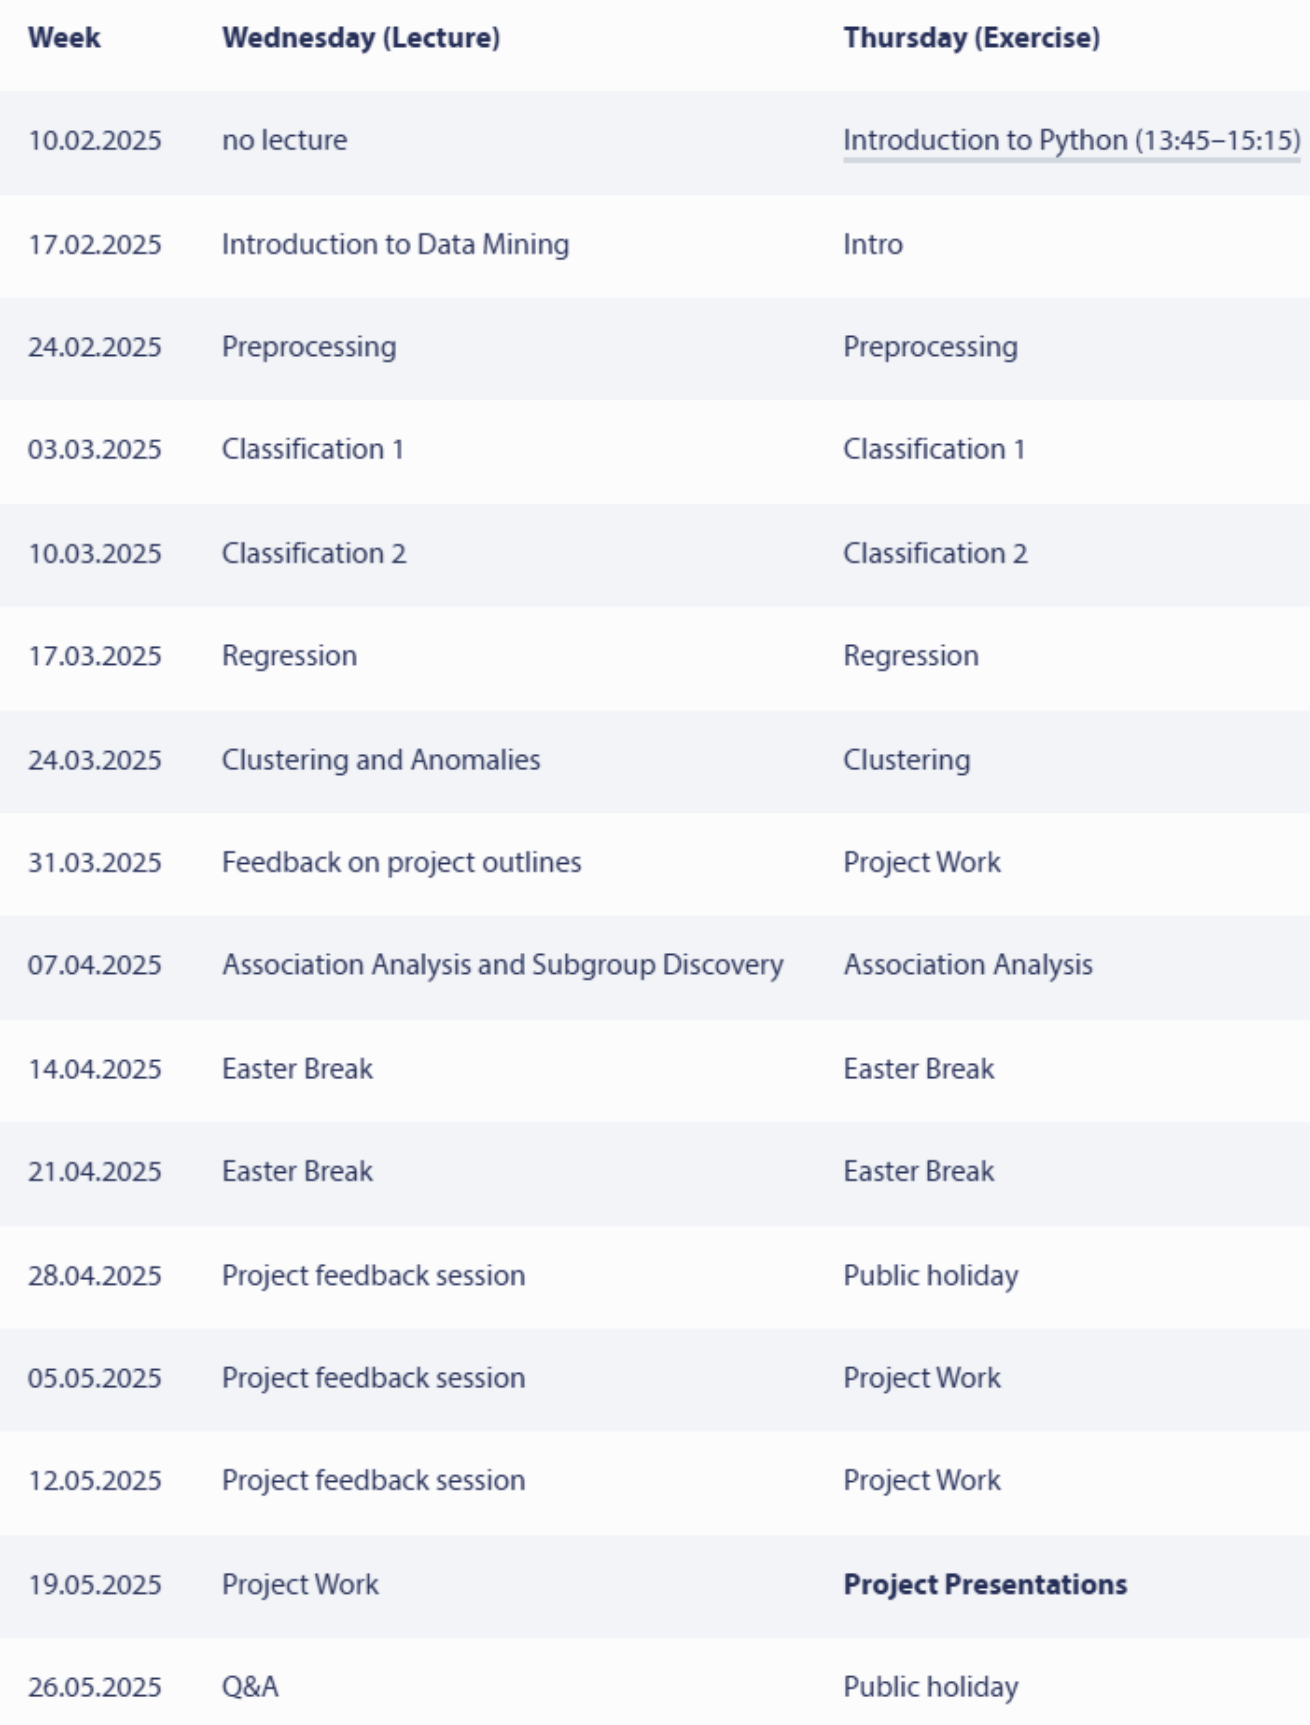
\includegraphics[width=\textwidth,height=4.6cm,keepaspectratio]{images/img_p15_1_90.png}
\end{center}
\end{column}
\end{columns}
\end{frame}

% Slide 16: Textbooks for the Course
\begin{frame}{کتاب‌های مرجع درس}
\begin{columns}[T,onlytextwidth]
\begin{column}{0.65\textwidth}
\begin{itemize}
  \item \textbf{کتاب اصلی داده‌کاوی:}
  \begin{itemize}
    \item \lr{Pang-Ning Tan, Michael Steinbach, Vipin Kumar}
    \item \lr{Introduction to Data Mining}, \lr{2nd Edition}
    \item انتشارات \lr{Pearson / Addison Wesley}
  \end{itemize}
  \vspace{0.2cm}
  \item \textbf{کتاب عملی یادگیری ماشین:}
  \begin{itemize}
    \item \lr{Aurélien Géron}
    \item \lr{Hands-on Machine Learning with Scikit-Learn, Keras \& TensorFlow}
    \item ویرایش دوم یا سوم، انتشارات \lr{O'Reilly}، \lr{2019} یا \lr{2022}
  \end{itemize}
  \vspace{0.2cm}
  \item \textbf{مستندات پایتون:}
  \begin{itemize}
    \item \lr{\footnotesize https://scikit-learn.org/stable/user\_guide.html}
  \end{itemize}
\end{itemize}
\end{column}
\begin{column}{0.32\textwidth}
\begin{center}
  
\includegraphics[width=0.85\textwidth,height=2.3cm,keepaspectratio]{images/img_p16_1_94.jpeg}\\[0.15cm]
  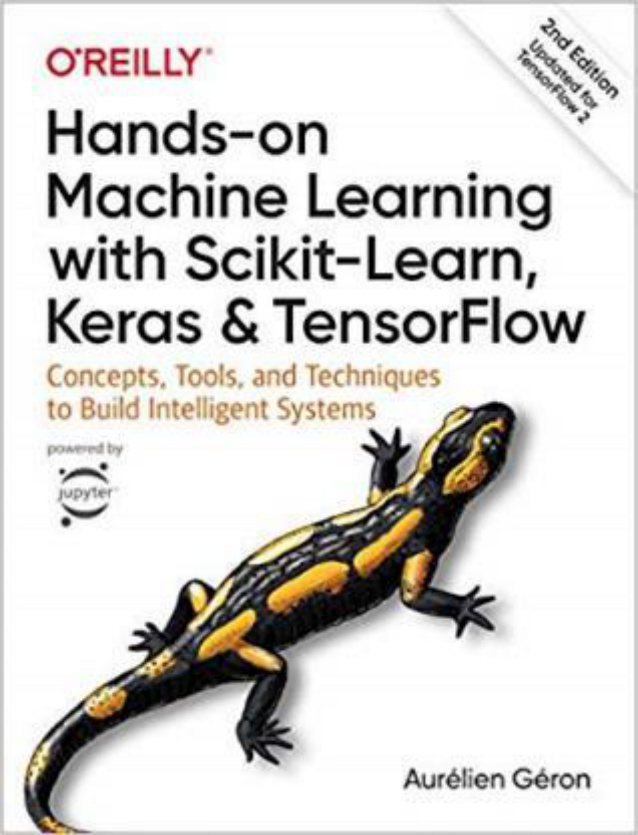
\includegraphics[width=0.85\textwidth,height=2.3cm,keepaspectratio]{images/img_p16_2_95.jpeg}
\end{center}
\end{column}
\end{columns}
\end{frame}

% Slide 17: Videos and Screencasts
\begin{frame}{ویدیوها و ضبط‌های آموزشی}
\begin{itemize}
  \item \textbf{ویدیوهای ضبط‌شده کلاس‌ها و تمرین‌ها:}
  \begin{itemize}
    \item پیوند: \lr{https://www.uni-mannheim.de/dws/teaching/lecture-videos} (نیازمند اتصال به \lr{VPN} دانشگاه)
    \item ویدیوهای درس تئوری توسط هایکو پاولهایم (\lr{HWS 2020}) و کریستین بیتزر (\lr{FSS 2020})
    \item ویدیوهای حل تمرین توسط رالف پیترز (\lr{FSS 2022})
  \end{itemize}
  \vspace{0.2cm}
  \item \textbf{یادآوری مهم:} اسلایدها و سرفصل‌ها سالانه بازنگری می‌شوند؛ لذا مباحث کلاس فعلی ملاک ارزیابی است.
\end{itemize}
\begin{center}
  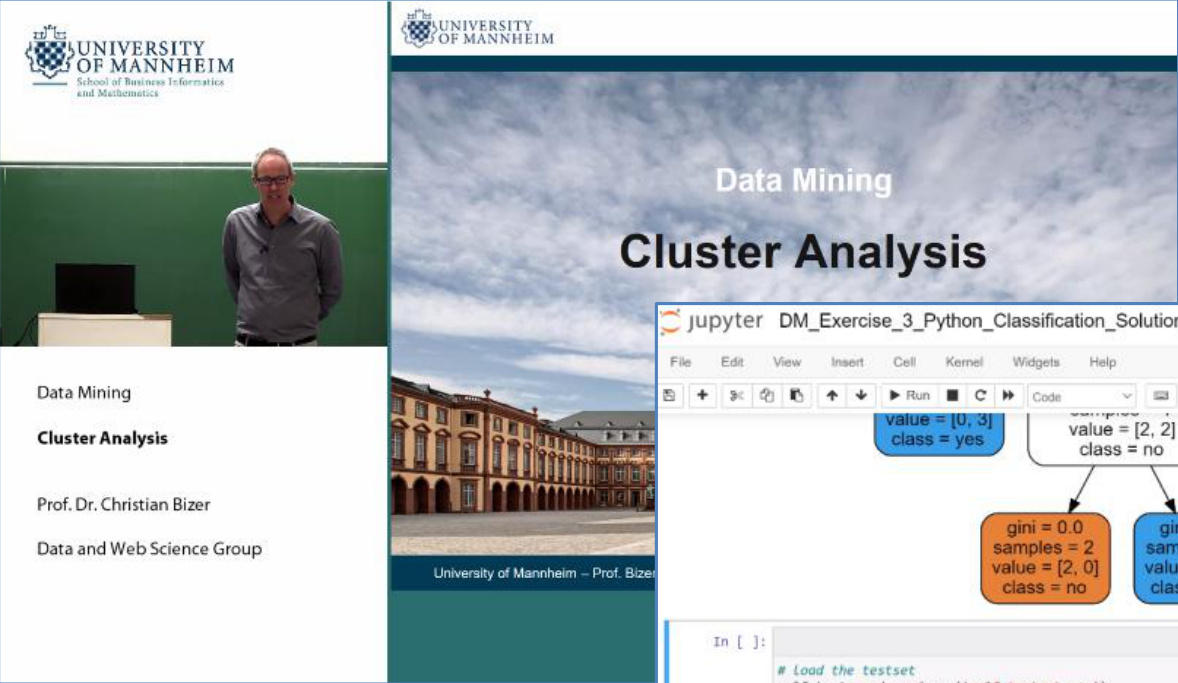
\includegraphics[height=1.8cm]{images/img_p17_1_99.jpeg}\hspace{0.2cm}
  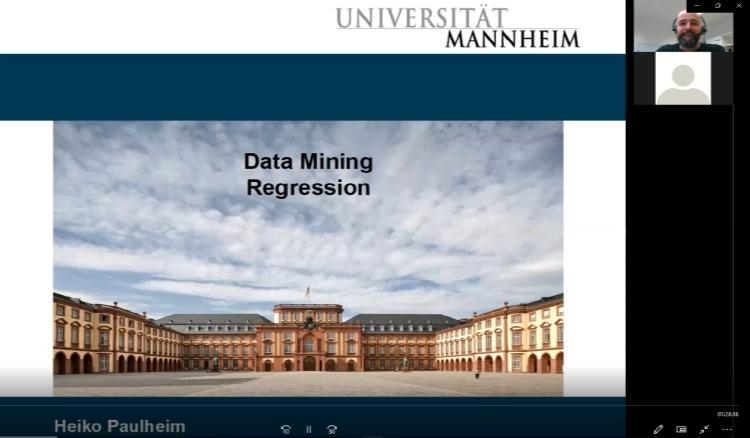
\includegraphics[height=1.8cm]{images/img_p17_2_100.jpeg}\hspace{0.2cm}
  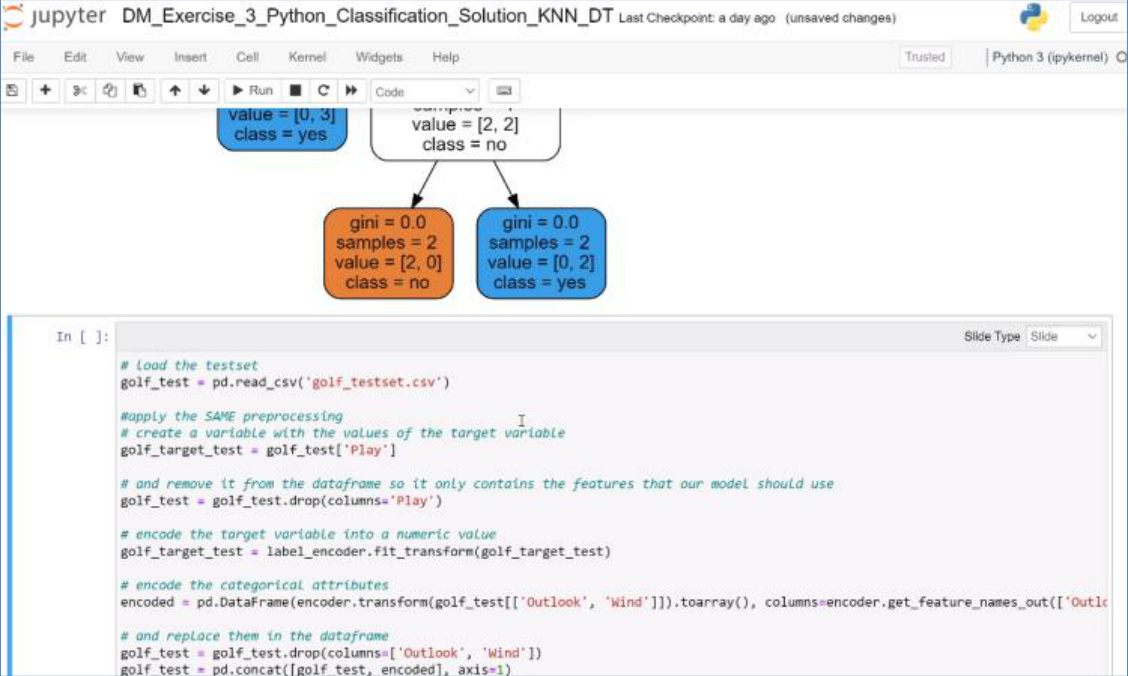
\includegraphics[height=1.8cm]{images/img_p17_3_101.jpeg}
\end{center}
\end{frame}

% Slide 18: Questions?
\begin{frame}{پرسش و پاسخ}
\begin{center}
  \vspace{0.4cm}
  {\fontsize{18}{22}\selectfont\color{mannheimblue}\textbf{آیا درباره ساختار درس سؤالی دارید؟}}\\[0.5cm]
  
\includegraphics[width=0.55\textwidth,height=3.8cm,keepaspectratio]{images/img_p18_2_104.jpeg}
\end{center}
\end{frame}
